\documentclass[11pt]{report}
\usepackage{geometry}
\geometry{letterpaper, top=1in, bottom=1in, left=1in, right=1in}                                 
\usepackage[parfill]{parskip}   
\usepackage{graphicx}
\usepackage{amssymb}
\usepackage{epstopdf}
\usepackage{array}
\usepackage{tabularx}
\setlength{\parindent}{0em}
\pagenumbering{gobble}

\DeclareGraphicsRule{.tif}{png}{.png}{`convert #1 `dirname #1`/`basename #1 .tif`.png}

\newcommand{\newday}[1]{\newpage{\LARGE \textbf{#1}}\\}
\newcommand{\imagefolder}{/Users/lauriaclarke/Documents/mfadt/ms1/lauriaclarke.github.io/instructionsetsforstrangers}


\title{INSTRUCTION SETS FOR STRANGERS -- PART I}
\date{}       
                                   
\begin{document}
\maketitle
%\tableofcontents
%----------------------------------------------
\section*{Location Choice}

After some discussion, we decided that a crosswalk would be the most exciting place to observe interactions between strangers. Given the high degree of randomness in who you encounter while crossing the street it seemed like an interesting choice -- particularly if the goal is to foster interaction between strangers. 

To pick a crosswalk we walked along 17th street between 5th and 2nd avenues. 

On the northeast corner of Union Square Park we discovered a crosswalk that included a median area. Few crosswalks in Manhattan cross two-way traffic -- this crosswalk crosses Park Ave. which is two lanes of divided and opposing traffic. Overall, this has the effect of making the intersection much larger and the act of walking across the street is much longer. 

\begin{figure}[ht]
\centering
\includegraphics[scale=0.10, angle=270]{"images/crosswalk_nopeople.jpg"}
\caption{The selected crosswalk on 17th st.}
\label{fig:nopeople}
\end{figure}

% insert history about Union Sq Park here

\section*{Initial Observation}

After walking by the first time around 4 PM on a weekday, we decided to return on a Saturday at noon -- during the Farmer's Market. The area surrounding Union Square is heavily trafficked on weekdays by commuters going to or from the train. Our hope for the weekend, was that more people would be paying attention to their surroundings and less focused on getting where they needed to go quickly. After completing a the AEIOU exercise at the intersection, this generally seemed to be true. Most people crossing the street were shopping at the market and spending time with friends. 

\begin{figure}[ht]
\centering
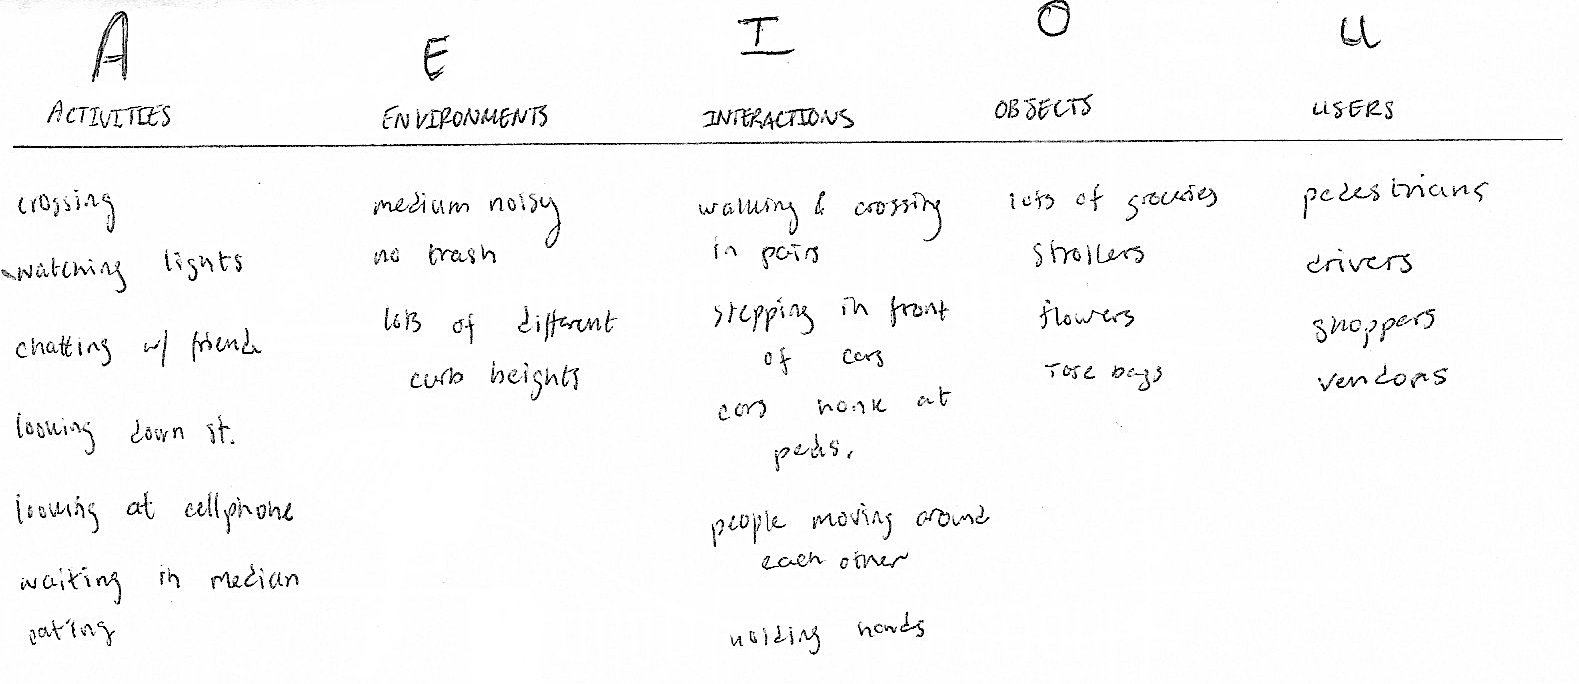
\includegraphics[scale=0.8]{"images/ms1_aeiou.png"}\\

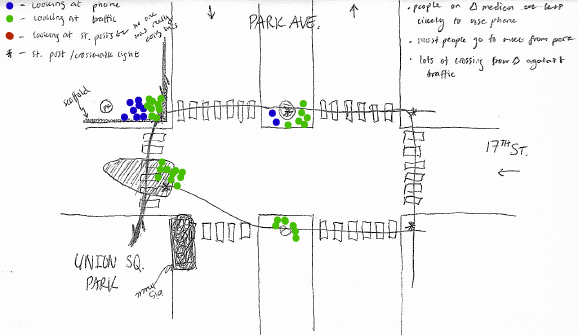
\includegraphics[scale=0.8]{"images/ms1_behaviormap.png"}
\caption{AEIOU and Behavior mapping exercise}
\label{fig:behaviormap}
\end{figure}

Behavior mapping at the crosswalk revealed some more interesting data. People waiting at the crosswalk were generally found to be doing one of three things: chatting with a friend, looking at their phone, or looking at traffic. The majority of people waiting at the intersection spent their time looking at traffic. I think this may be due to the fact that this intersection is quite long -- it has a median -- and cars moving down Park Ave. tend to be going pretty fast. It seems like an intersection that requires attention as a pedestrian.  

Since most of the people crossing the street here were travelling to or from the farmer's market and many were with fiends or family, the majority of foot traffic was routed over the small delta in the bike lane (see shaded shape in map) with people clustered in groups. In comparison, few people stopped on the medians in Park Ave. Those that did were generally alone and walking out of sync with the lights and were paying attention to traffic, not their cellphones.


\section*{Ideation}

After collecting data, we began to brainstorm about which interactions would be most interesting between strangers crossing the street. The idea of playing a simple game with a strange on the other side of the crosswalk was very appealing, but most required more synchronization and direction than was possible in such a short amount of time (the amount of time spent waiting at the crosswalk).
 
\begin{figure}[ht]
\centering
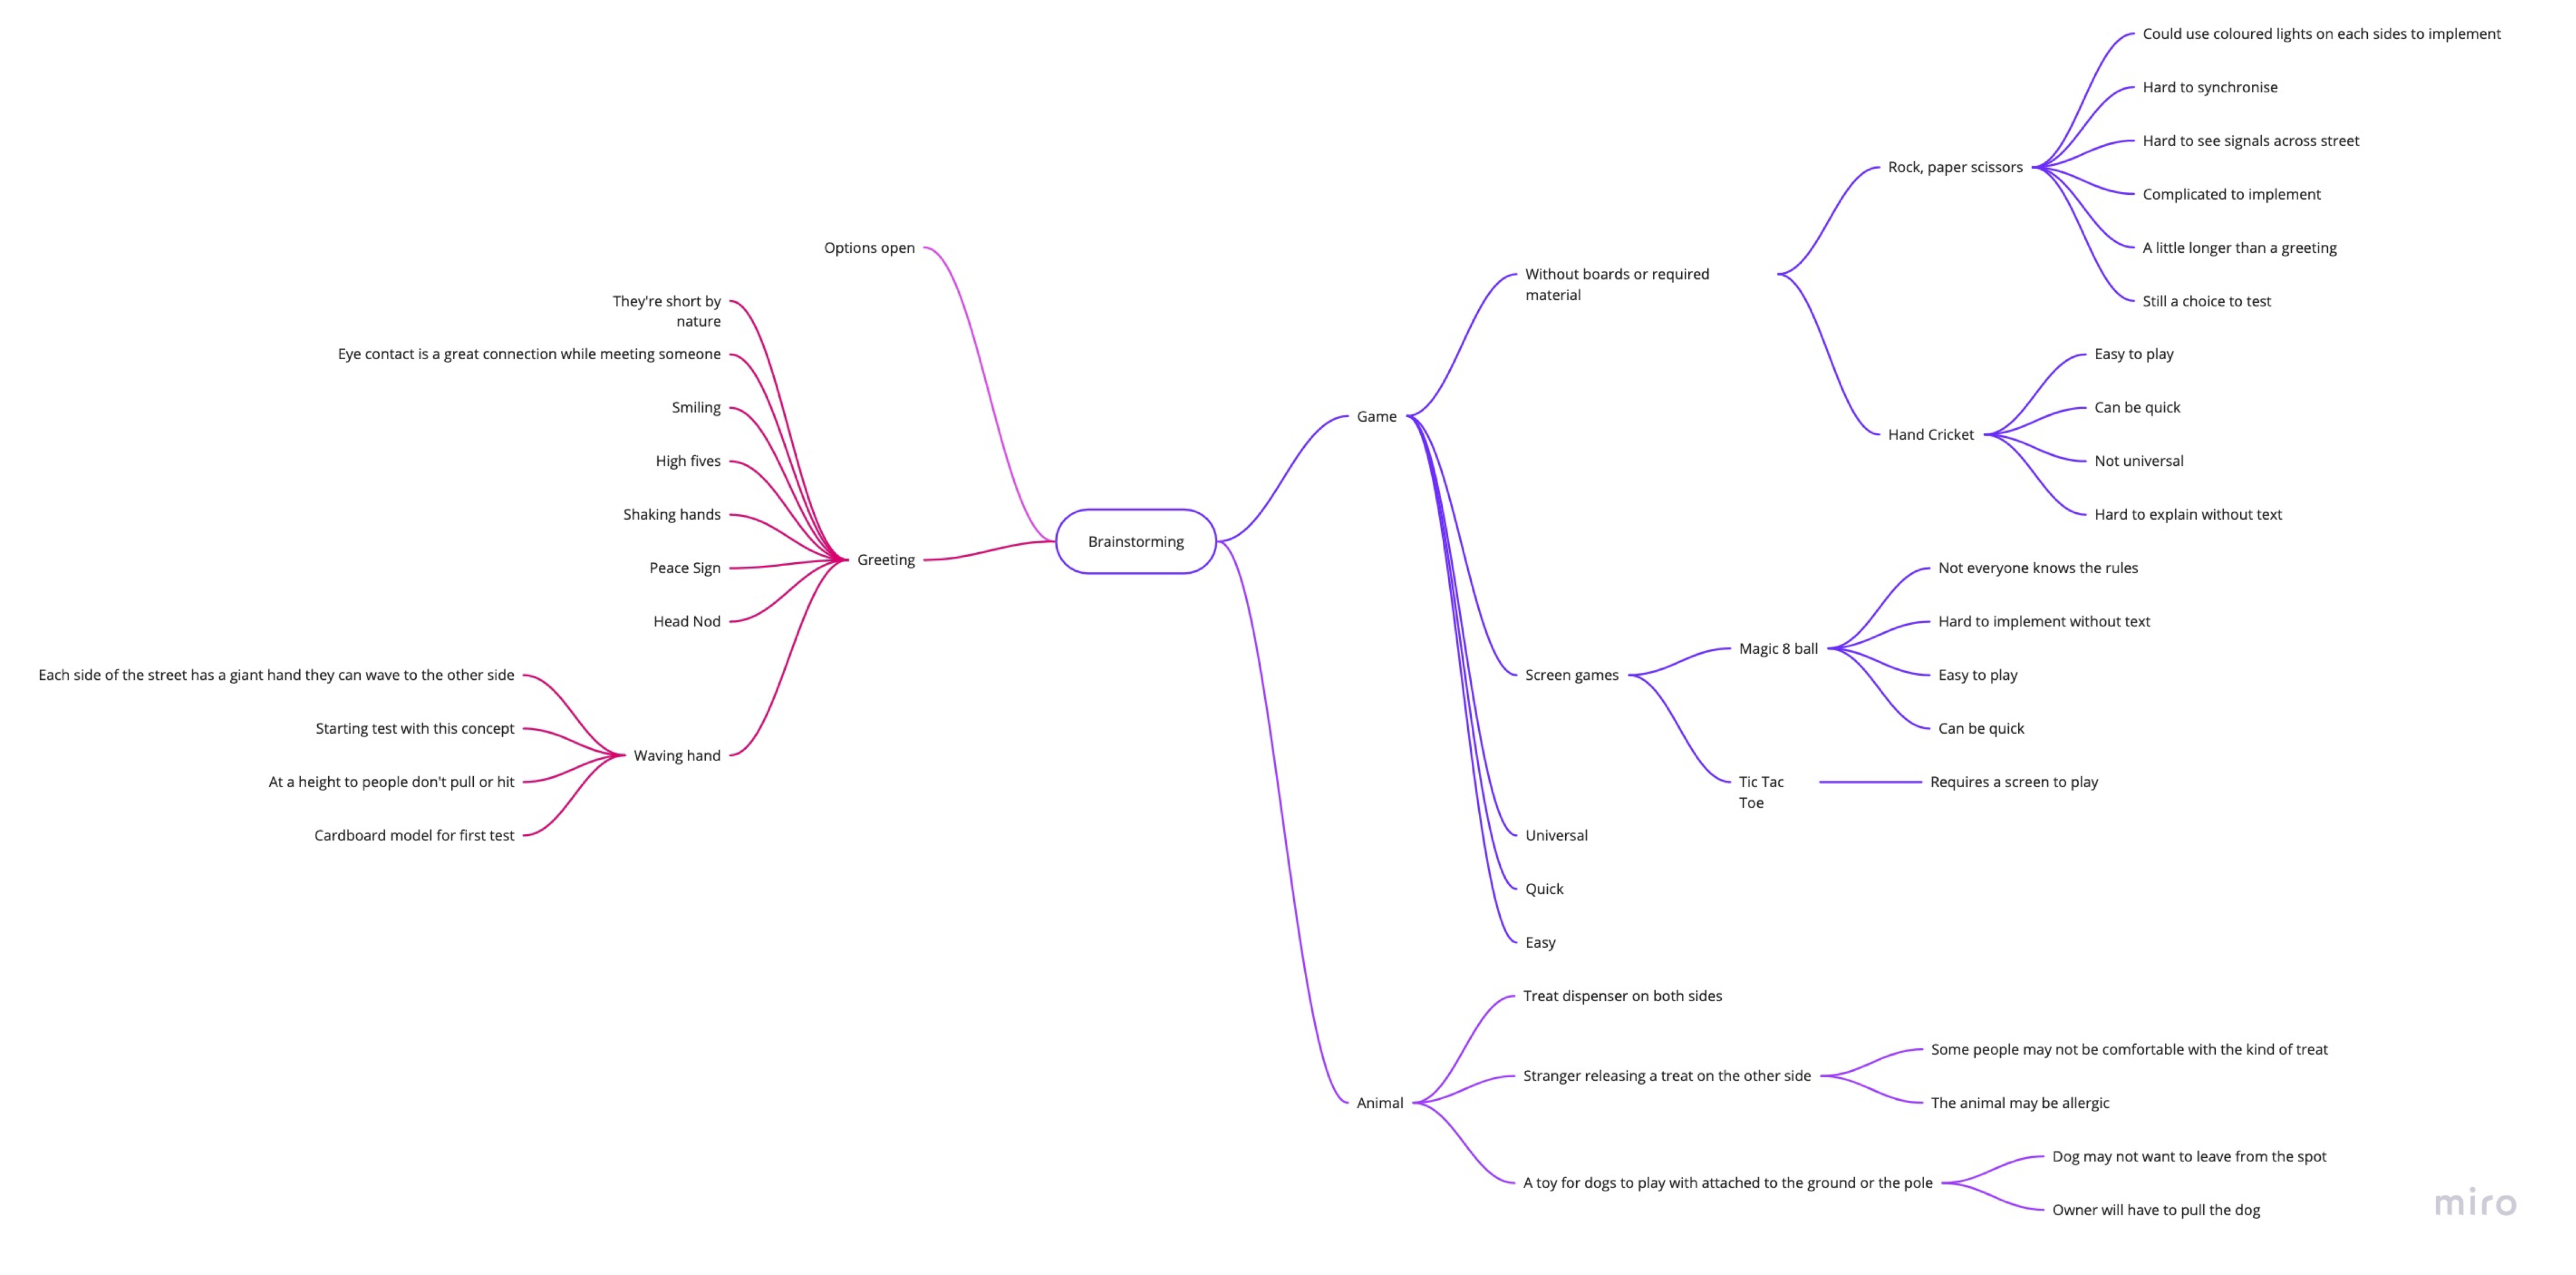
\includegraphics[width=1.4\textwidth, angle=90]{"images/ms1_brainstorming.png"}
\caption{Results of brainstorming activity.}
\label{fig:brainstorm}
\end{figure}

After deciding that the ideal interaction would be really quick -- such as a greeting -- we began thinking about fun ways to wave at someone on the other side of the street. The idea of having a giant arm and hand on each side of the street was very appealing and seemed both simple and effective. The below sketch illustrates what a pair of hands / arms would look like on location.
 
\begin{figure}[ht]
\centering
\includegraphics[scale=0.08]{"images/wavemachine_overlay_2.jpg"}
\caption{Sketch of device on location.}
\label{fig:overlay}
\end{figure}

The best part of such a contraption is that it would not necessarily require the use of electronics. Using thin plywood, springs and some clever balancing, we could create the arm mechanism from very basic materials. Below is a sketch of one possible mechanism.
 
\begin{figure}[ht]
\centering
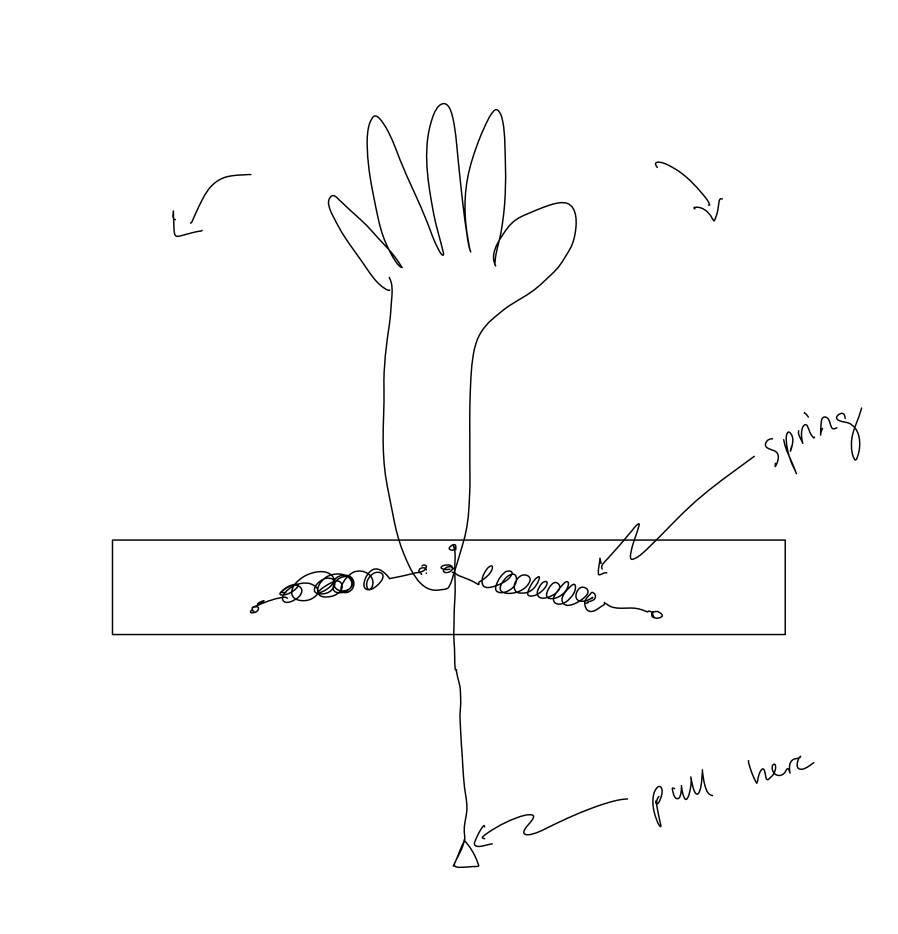
\includegraphics[scale=0.6]{"images/wavemachine_sketch.png"}
\caption{Possible mechanical design of device.}
\label{fig:sketch}
\end{figure}





\end{document}
